%! TeX program = lualatex
\documentclass[../main.tex]{subfiles}
\begin{document} \section{Review of piecewise-defined functions}
  A piecewise-defined function are defined using different equations for different parts of their domain. 
  \blanklines{5}

  We use the ``left brace'' notation to define piecewise-defined (or just piecewise) functions. 

  \begin{example}
    The absolute function is a piecewise function whose definition is
    \[
      |x| = 
      \begin{cases}
        x, &\text{if } x > 0, \\
        0, &\text{if } x = 0, \\
        -x, &\text{if } x < 0.
      \end{cases}
    \]
  \end{example}

  \begin{example}
    Sketch the function

    \begin{minipage}{2in}
    \[
      f(x) = 
      \begin{cases}
        x + 1, &x > 3 \\
        4, &x < 3
      \end{cases}
    \]
    \end{minipage}
    \begin{minipage}{5in}
      \centering
      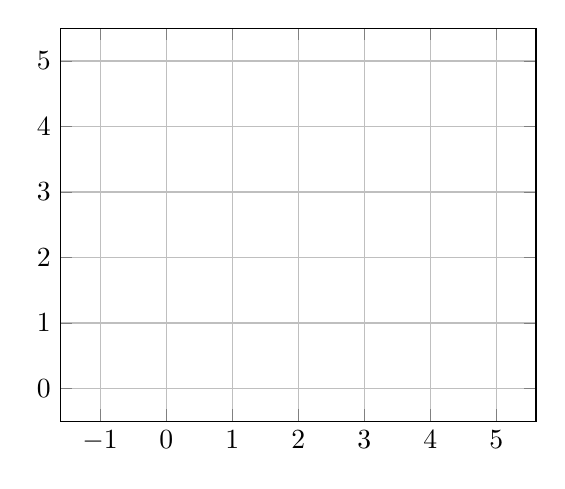
\begin{tikzpicture}
        \begin{axis}[xmin=-1, xmax=5, ymin=0, ymax=5, grid=major, width=3in, xtick={-1,0,...,5}, ytick={0,1,...,5}, enlargelimits=true]
        \end{axis}
      \end{tikzpicture}
    \end{minipage}
  \end{example}

  \begin{example}
    The graph of a function \(g(x)\) is given below. Write down the definition of \(g(x)\) as a piecewise function. Assume the domain of \(g(x)\) is \([-2, 5]\).

    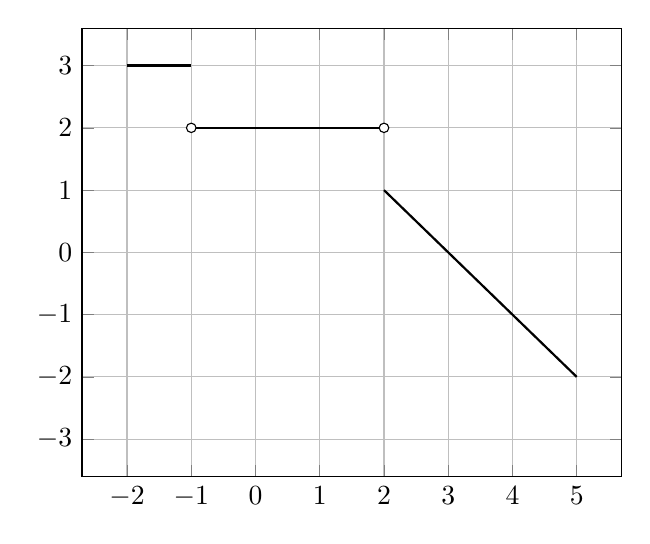
\begin{tikzpicture}
      \begin{axis}[
        enlargelimits=true,
        xmin=-2, xmax=5,
        ymin=-3, ymax=3,
        xtick={-2,-1,...,5},
        ytick={-3,-2,...,3},
        grid=major,
        ]
        \addplot[thick] coordinates {(-2, 3) (-1,3)};
        \addplot[thick] coordinates {(-1, 2) (2, 2)};
        \addplot[thick] coordinates {(2, 1) (5, -2)};
        \draw[fill=white] (axis cs:-1,2) circle (0.075);
        \draw[fill=white] (axis cs:2,2) circle (0.075);
      \end{axis}
      
    \end{tikzpicture}
  \end{example}
  

\end{document}
